%% document class
\documentclass[10pt]{beamer}
%%theme
\usetheme[hideothersubsections]{Berkeley}
%% page settings
%\usepackage[space,noindent]{ctex}
\usepackage{xcolor}
\usenavigationsymbolstemplate{}

%% packages
\usepackage{tikz}
\usepackage{geometry}

%%color settings
%%%%% Color Schema

\definecolor{blue_dark}{RGB}{38,50,56}
\definecolor{blue}{RGB}{33,150,243}
\definecolor{blue_light}{RGB}{79,195,247}
\definecolor{grey_dark}{RGB}{38,50,56}
\definecolor{grey}{RGB}{33,150,243}
\definecolor{grey_light}{RGB}{33,150,243}

%% theme settings
\setbeamercolor*{palette primary}{fg=grey_dark,bg=blue_light} % upper part
\setbeamercolor*{palette secondary}{fg=grey_dark,bg=blue_light} % left part (background)
\setbeamercolor*{sidebar left}{fg=blue_light,bg=grey_dark} % left part with links
\setbeamercolor*{palette sidebar primary}{fg=blue_light}
\setbeamercolor*{palette sidebar secondary}{fg=blue_light}

%% new commands
%\input{settings/macros}
\addtobeamertemplate{frametitle}{\vskip+0.6ex}{}
\makeatletter
\beamer@headheight=2\baselineskip
\makeatother

\begin{document}

\author[Group 9]{Suvojit Manna\\Pronab Mukherjee\\Barun Gupta\\Somnath Rakshit\\}
\title[Machine Learning]{Introduction to Machine Learning using \LaTeX}
%\logo{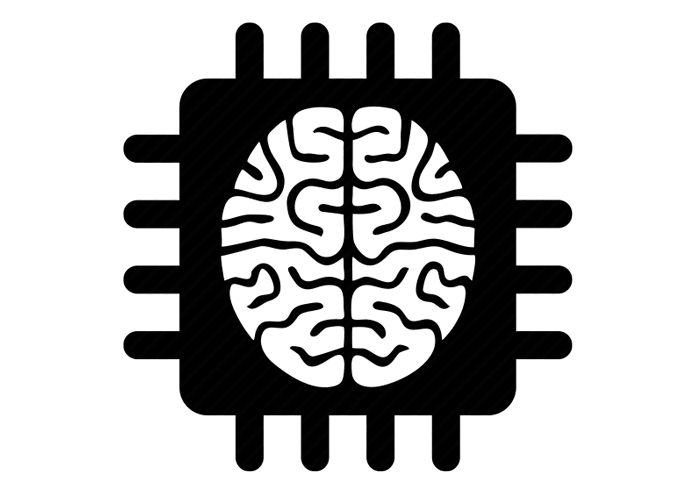
\includegraphics[width=4mm]{images/icon}}
\institute[JGEC]{Jalpaiguri Govt Engineering College}
%\date{City, date}


%% Title Page
\begingroup
\setbeamercolor{background canvas}{bg=blue_dark}
\begin{frame}[plain,t]
\hspace*{-22 mm}

\includegraphics[width=\paperwidth,height=\paperheight]{images/ml_bg}
\end{frame}
\endgroup

%% A Team Page
\begingroup
\usebackgroundtemplate{%
\tikz\node[opacity=0.3] {
\includegraphics[height=\paperheight,width=\paperwidth]{images/bg-vec}}
;}
\begin{frame}[t]{The A Team}

\Huge{Presented By:\\}
\large{~\\Suvojit Manna\\Pronab Mukherjee\\Barun Gupta\\Somnath Rakshit\\}
\end{frame}
%% contents
\begin{frame}{Contents in Brief}
%\tableofcontents
\tableofcontents[hideallsubsections]
\end{frame}
\endgroup
%% Big Font Page: Lets get started
\begingroup
\setbeamercolor{background canvas}{bg=blue_dark}
\setbeamercolor{normal text}{fg=blue_light}
\begin{frame}[plain,c]
\hspace*{10 mm}
\vspace*{-18 mm}
\textcolor{blue_light}{\Huge{Let's Get Started}}
\end{frame}
\endgroup


\begingroup
\usebackgroundtemplate{%
\tikz\node[opacity=0.3] {
\includegraphics[height=\paperheight,width=\paperwidth]{images/bg-vec}}
;}

\section{Introduction}
\begin{frame}{Introduction | Machine Learning}
\end{frame}
\subsection{Getting to know}
\begin{frame}{Getting to know | Machine Learning}
\end{frame}
\subsection{Benefits}
\begin{frame}{Benefits | Machine Learning}
\end{frame}
\subsection{Case Studies}
\begin{frame}{Case Studies | Machine Learning}
\end{frame}
\subsection{Applications}
\begin{frame}{Applications | Machine Learning}
\end{frame}

\section{Regression}
\begin{frame}{Introduction | Regression}
\end{frame}
\subsection{Usages}
\begin{frame}{Usages | Regression}
\end{frame}
\subsection{Benefits}
\begin{frame}{Benefits | Regression}
\end{frame}
\subsection{Example Cases}
\begin{frame}{Example Cases | Regression}
\end{frame}

\section{Classifications}
\begin{frame}{Introduction | Classifications}
\end{frame}
\subsection{Usages}
\begin{frame}{Usages | Classifications}
\end{frame}
\subsection{Example Cases}
\begin{frame}{Example Cases | Classifications}
\end{frame}


\section{Deep Learning}
\begin{frame}{Introduction | Deep Learning}
\end{frame}
\subsection{Neural Networks}
\begin{frame}{Neural Networks | Deep Learning}
\end{frame}
\subsection{Meaning}
\begin{frame}{Meaning | Deep Learning}
\end{frame}
\subsection{Usages}
\begin{frame}{Usages | Deep Learning}
\end{frame}
\subsection{Advantages}
\begin{frame}{Advantages | Deep Learning}
\end{frame}



\section{Conclusion}
\begin{frame}{The pain is almost over}
\end{frame}
\begin{frame}{Bibliography}
\end{frame}
\endgroup

\begingroup
\setbeamercolor{background canvas}{bg=blue_dark}
\setbeamercolor{normal text}{fg=blue_light}
\begin{frame}[plain,c]
\hspace*{10 mm}
\vspace*{-18 mm}
\textcolor{blue_light}{\Large{Now that was very interesting!}}
\end{frame}
\begin{frame}[plain,c]
\hspace*{30 mm}
\vspace*{-20 mm}
\textcolor{blue_light}{\Large{The End}}
\end{frame}
\endgroup

\end{document}


